\documentclass[12pt]{paper}
\usepackage{setspace}
\usepackage{graphicx}
\usepackage{lineno}
\usepackage[style=numeric-comp,url=false,doi=false,isbn=false,maxnames=2,maxbibnames=2,firstinits,sorting=none]{biblatex}
\bibliography{/Users/DGravel/Documents/library.bib}

\title{Resource-ratio theory in metaecosystems}

\begin{document}

%\title{Resource-ratio theory in metaecosystems}

\author{Dominique Gravel}

\maketitle\onehalfspacing\linenumbers

\begin{abstract}
Background: Tilman's theory is intrinsically spatial. Predictions: increasing variance in resource supply ratios promote diversity and increasing fertility reduces diversity 
Question: What's happening when we add dispersal?
Approach: metaecosystem, dispersal of nutrients, plants and detritus
Key results: all flows are homogeneizing but have unique consequences. Nutrient dispersal decreases the variance . Producer dispersal influences the ZNGI. Detritus dispersal displace the supply points with an enrichnment. These flows thus affect the conditions for coexistence and diversity. Could also result in alternate stable states
Conclusion
\end{abstract}

\keywords{consumer-resource, metaecosystems, dispersal, resource-ratio, stoichiometry, spatial ecology, coexistence}

%========================================================%
\section{Introduction}


Paragraph 1: contribution of the resource-ratio theory to the understanding of coexistence

Paragraph 2: resource-ratio theory is essentially spatial, but has yet to integrate recent developments of metacommunity theory. Only a few amounts of papers deals with spatial exchanges of nutrients and organisms (Klausmeier; Ryabov and Blasius). These studies concern the vertical distribution of biomass in the water column and do not provide a mechanistic understanding of the impacts of dispersal on coexistence.

Paragraph 3: objectives and approach 


%========================================================%
\section{Model description}
We consider a general metaecosystem model with nutrient cycling in a spatially heterogeneous landscape (Gravel et al. 2010). The model accounts for $n$ different inorganic nutrients $N_{jx}$ (where $j$ denotes a nutrient and $x$ a locality) and is stoichiometrically explicit by maintaining mass balance for each of them. Local dynamics follow the ecosystem model of Daufresne and Hedin (2005). The dynamics of the primary producers $P_{ix}$ of species $i$ follow:

%-----------------%
\begin{equation}
	\label{e:bnet}
	\frac{dP_{ix}}{dt}=G_{ix}(N_{1x},N_{2x},…,N_{nx})P_{ix}-m_{i}P_{ix}-\Delta_{Px}
\end{equation}
%-----------------%

where $G_{ix}$ is the growth function describing the per capita uptake rate of the inorganic nutrients and $m_{i}$ is the mortality rate. The total biomass of the primary producer species $i$ is given by the sum of all the nutrients bounded in its biomass, which are allocated in a constant ratio (quota): 

%-----------------%
\begin{equation}
	\label{e:bnet}
	q_{ij}=\frac{P_{ijx}}{\sum_{j=1}^{n}P_{ijx}}
\end{equation}
%-----------------%

The growth function $G_{ix}$ depends on the stoichiometry of the inorganic nutrients and the primary producer specific demand. We assume that $G_{ix}$ follows a Liebig’s law of the minimum:

%-----------------%
\begin{equation}
	\label{e:bnet}
	G_{i}=MIN\{\frac{g_{ij}(N_{j})}{q_{ij}}\}
\end{equation}
%-----------------%

where $g_{ij}$ represents the growth of the primary producer species $i$ when limited by nutrient $j$. We do not specify at this point the shape of the functional response. We consider a simple diffusive (passive) dispersal between compartments $C$ of the locality $x$ and its adjacent locality $y$: 

%-----------------%
\begin{equation}
	\label{e:bnet}
	\Delta_{Cx}=d_{C}(C_{x}-C_{y})
\end{equation}
%-----------------%

where $d_{C}$ is the diffusion rate of compartment $C$ between localities.  

Dead organic matter is directly incorporated in the detritus compartment $D_{ix}$, and then mineralized by decomposers at rate $r$:

%-----------------%
\begin{equation}
	\label{e:bnet}
	\frac{dD_{ix}}{dt}=m_{i}P_{ix}-rD_{ix}-\Delta_{Dx}
\end{equation}
%-----------------%

We do consider similar recycling rates among the different nutrients to maintain the simplicity of the analysis, but it is possible to expand the model to account for different recycling rates (see Daufresne and Hedin, 2005). 

The dynamics of the inorganic nutrient concentration accounts for external inputs, losses, recycling of detritus $D_{ix}$, consumption by primary producers $P_{ix}$ and diffusion among localities: 

%-----------------%
\begin{equation}
	\label{e:bnet}
	\frac{dN_{jx}}{dt}=S_{jx}-eN_{jx}-\sum_{i=1}^{s}q_{ij}G_{ix}N_{jx}+\sum_{i=1}^{s}r(1-\phi)D_{ix}-\Delta_{Nx}
\end{equation}
%-----------------%

The inorganic nutrients are supplied to each locality via mineral alteration and atmospheric depositions at rate $S_{jx}$, and leached out of the system at rate $e$. A fraction $\phi$ of the inorganic mineral is loss out of the system during the mineralization process.

%========================================================%
\section{Graphical interpretation of resource ratio theory}

The conditions for coexistence of primary producer species competing for two resources is best understood using a graphical representation of the model (Tilman, 1982). We first illustrate and derive tools to interpret the equilibrium state of the system with a single resident primary producer species and detritus mineralization at a single locality. We introduce dispersal for each compartment at the following section. 

The external supply point $S$ represents the equilibrium nutrient concentration in the system in absence of this primary producer (no consumption – Fig. 1A). The zero net growth isocline ($ZNGI_i$) represents the combination of the two nutrient levels ($N_{j}^*$) at which the growth of primary producer $i$ is null. The growth of the primary producer is possible only if the supply point is located above the $ZNGI_i$. 

The use of vectors is a convenient tool to understand the dynamics of the system and its equilibrium state. The mass balance constraint implies the system will satisfy the following conditions at equilibrium (denoted by the hat, assuming no dispersal):

%-----------------%
\begin{equation}
	\label{e:bnet}
	\widehat{G} _{ix}= m_{i} 
\end{equation}

\begin{equation}
	\label{e:bnet}
	m_{i}\widehat{P}_{ix}=r\widehat{D}_{ix} 
\end{equation}

\begin{equation}
	\label{e:bnet}
	S_{jx}-e\widehat{N}_{jx}=\sum_{i=1}^{s}q_{ij}\widehat{G}_{ix}\widehat{N}_{jx}-\sum_{i=1}^{s}r(1-l)\widehat{D}_{ix}
\end{equation}
%-----------------%

The condition at Eq. 7 defines the $ZNGI_i$ on the two-dimensional space of nutrients (growth is equal to mortality). The condition at Eq. 8 implies that at equilibrium, the accumulation of dead organic matter equals detritus recycling. The condition at Eq. 9 implies that the consumption of inorganic nutrients must equal the rate at which they are supplied. The primary producer consumes the two nutrients simultaneously, at the rate indicated by a consumption vector $\overrightarrow{c}_{x} = (-q_{i1}\widehat{G}_{ix}\widehat{N}_{1x},-q_{i2}\widehat{G}_{ix}\widehat{N}_{2x})$. The slope of the consumption vector is equal to the quota of the primary producer ($\alpha_{i}=q_{i2}/q_{i1}$, Fig. 1A). At equilibrium, the inorganic nutrient concentration is located along the ZNGI (Fig. 1A), at the point satisfying the following condition:

%-----------------%
\begin{equation}
	\label{e:bnet}
	\overrightarrow{u}_{x}+\overrightarrow{c}_{x}=\overrightarrow{0}
\end{equation}		 	
%-----------------%

where $\overrightarrow{u}_{x}=(S_{1x}-e\widehat{N}_{1x},S_{2x}-e\widehat{N}_{2x})$ is the inorganic nutrient supply vector. The inorganic nutrient concentration at equilibrium is found at the location where the projection of the consumption vector crosses the supply point (Fig. 1A). 

	The mineralization of the detritus pool alters the equilibrium density of the primary producer because it increases the overall nutrient supply. The inorganic nutrient consumption consequently increases, and potentially the inorganic nutrient concentration (Daufresne and Hedin, 2005). We must therefore consider an altered inorganic nutrient supply vector to balance the new consumption vector:

%-----------------%
\begin{equation}
	\label{e:bnet}
	\overrightarrow{u'}_{x}+\overrightarrow{c}_{ix}=\overrightarrow{0}
\end{equation}
%-----------------%

where $\overrightarrow{u'}_{x}$ is an altered nutrient supply vector. The consumption vector therefore points toward a net nutrient supply point $S'_{x}$, which his new location is given by:

%-----------------%
\begin{equation}
	\label{e:bnet}
	S'_{jx}=\sum_{i=1}^{s}q_{ij}G_{ix}P_{ix}e^{-1}+N_{jx}
\end{equation}
%-----------------%

The location of the net supply point $S'$ will simply be a translation of the original supply point $S$ along the projection of the consumption vector when the mineralization of the detritus returns nutrients to the inorganic pool in the same proportion than they are sequestered in the biomass (i.e. following the quota $q_{i}$, Daufresne and Hedin, 2005). 

	The location of the net nutrient supply point $S'$ is crucial to understand the impacts of nutrient cycling and diffusion on coexistence. Remember the criterion for coexistence in the classical resource-ratio theory is that i) the supply point must be located between the projection of the consumption vectors of the competing species (Fig. 1B) and ii) that species are more limited by the resource they consume the most (in other words, the species with the uppermost ZNGI also has the steepest consumption vector). The addition of nutrient recycling alters this condition: it is the net nutrient supply point $S'$ that must be located between the projection of the consumption vectors in order to have coexistence (Daufresne and Hedin, 2005). 

%========================================================%
\section{Metaecosystem dynamics}

The fundamental criteria for stable coexistence to occur between two species is reciprocal invasibility when one of the species is at equilibrium (the resident) and the other species is rare. In this section we therefore analyse the impacts of spatial flows between two ecosystems on the equilibrium inorganic nutrient concentration in the presence of a single resident primary producer. We focus on the location of the net supply point because it is central to understand invasion conditions (equilibrium inorganic nutrient concentration) and thus coexistence in both locations. Stable coexistence between two species will be possible when each of them has a positive per capita growth rate when at low abundance (Chesson, 2000; Gravel et al. 2011). In terms of graphical representation of the dynamics, it means that the equilibrium nutrient concentration of each species when resident will be above the ZNGI of the invader. We study each spatial flow independently, even though they are likely to be colinear in nature, in order to distinguish their isolated effect on coexistence. We finish with the analysis of a special case where spatial flows and nutrient recycling promote unstable coexistence (alternate stable states) between two competing species. The analysis is essentially derived from a graphical interpretation of equilibrium vectors.

%===============================%
\subsection{Case 1: Detritus diffusion}

Because we assume passive diffusion, the detritus will flow from the most productive location to the least productive one (Gravel et al., 2010a,b). The equilibrium total biomass of the producer at a location, and consequently the detritus biomass producer, is easily found on the two-dimensional space of nutrients (Fig. 2). The biomass will be proportional to the distance between the net supply point and the equilibrium inorganic nutrient concentration (in absence of diffusion). For instance, at Fig 2, the equilibrium producer and detritus biomass will be larger at the grey location (the most productive combinations of the two resources) than the black location (the least productive). Because it is passive, diffusion between the two locations has an averaging effect, meaning that it will tend to homogenize the detritus compartments from the two locations. Detritus will move from the most productive (grey) to the least productive (black) location. Consequently the net supply rate of both nutrients increases at the least productive location  while it decreases at the least productive location. The movement of the net supply point still follows however the projection of the consumption vector because the two nutrients are exchanged between the location exactly in the same proportion they are consumed (the quota of the detritus is the same as the quota of the producer). The equilibrium inorganic nutrient concentration thus remains unchanged by spatial flows of detritus, and consequently coexistence is neither promoted or impeded by detritus flows.

	This result is easily shown with a simple derivation of the model. We calculate the displacement of the supply point ($\Delta S_{jx}$) of nutrient $j$ at location $x$ by comparing Eq. 10 and 11 and find:

%-----------------%
\begin{equation}
	\label{e:bnet}
	\Delta S_{jx}=q_{j}\phi r\widehat{D}_{x}e^{-1}
\end{equation}
%-----------------%

What is interesting is to understand if the position of the net supply point of one nutrients is more important than the other one. Taking the ratio of deltas (the slope of the displacement vector) yields a result between 0 (only the supply point of nutrient 2 is moving) and infinity (only the supply point of nutrient 1 is moving). Any ratio different from the slope of the consumption vector indicates a differential movement susceptible to influence coexistence. Considering the two nutrients, we find that the slope of the change (see Fig 1) is:

%-----------------%
\begin{equation}
	\label{e:bnet}
	Slope=\frac{q_{2}\phi r\widehat{D}_{x}e^{-1}}{q_{1}\phi r\widehat{D}_{x}e^{-1}}=\frac{q_{2}}{q_{1}}
\end{equation}
%-----------------%

which corresponds to the slope of the consumption vector (the ratio of quotas). Altough it does not influence stable coexistence, the spatial flow of detritus promotes unstable coexistence if the displacement of the net supply point from the original supply point is crossing the projection of an inferior competitor toward the coexistence area (see below), or alternatively it could lead to competitive exclusion if it moves in the opposite situation. 

%===============================%
\subsection{Case 2: Nutrient Dispersal}

The impact of nutrient diffusion on coexistence is somewhat more complicated because the two nutrients are not necessarily exchanged in the same ratio between locations. The results differ if the primary producer is limited by the same nutrient in the two locations, or by different nutrients, but the general principle remains the same (the latter is illustrated at Fig. 3): each of the inorganic nutrient will flow from the location with highest concentration to the location with the lowest (Gravel et al. 2010a), which will result in a spatial homogeneization of the net supply points. In other words, the net supply points will get closer in the two-dimensional space with increasing diffusion rate. At Fig. 3 for instance, the nutrient 1 has a greater concentration in the grey patch and will consequently flow toward the black patch (and the opposite for nutrient 2). The grey patch will thus be enriched in nutrient 2, while the black patch in nutrient 2. More generally, in the situation where the same nutrient is limiting the producer at the two locations, the location with the highest supply rate of the non-limiting nutrient will be the net exporter of that nutrient and the other location will be the net importer. Consequently the net supply point, the equilibrium nutrient concentration and the biomass will be more similar with increasing diffusion. In the situation where different nutrients are limiting the producer in the two locations, one nutrient will be exported (the non-limiting one) and one nutrient will be imported (the limiting one) at each location. Diffusion will also homogenize all compartments in this situation. 

	The equilibrium solution to the situation of nutrient dispersal is more complicated than for detritus, but still provides interpretable predictions.The displacement of the net supply point relative to the original supply point in this situation is:

%-----------------%
\begin{equation}
	\label{e:bnet}
	\Delta S_{jx}=q_{j}\phi m\widehat{P}_{x}^{-1}-\Delta_{Nx}
\end{equation}
%-----------------%

And thus the slope of the change for the supply point at location $x$ is:

%-----------------%
\begin{equation}
	\label{e:bnet}
	Slope=\frac{q_{2}\phi m\widehat{P}_{x}^{-1}-d_{N}(\widehat{N}_{2x}-\widehat{N}_{2y})}{q_{1}\phi m\widehat{P}_{x}^{-1}-d_{N}(\widehat{N}_{1x}-\widehat{N}_{1y})}
\end{equation}
%-----------------%

	This equation is already quite complicated and it is not possible to derive an instructive solution for the equilibrium nutrient concentration and producer densities in the two locations. This solution however simplifies considerably in the simpler, but still informative, situation where there is no nutrient recycling (i.e. $\phi = 1$ and $r = 0$):

%-----------------%
\begin{equation}
	\label{e:bnet}
	Slope=\frac{\widehat{N}_{2x}-\widehat{N}_{2y}}{\widehat{N}_{1x}-\widehat{N}_{1y}}
\end{equation}
%-----------------%

This equation is not complete in absence of the equilibrium inorganic nutrient concentrations, but these could be easily obtained from a graphical interpretation of equilibrium states (such as Fig. 3). As mentionned above, the relative position of the inorganic nutrient concentration at the two locations in absence of diffusion could be obtained graphically, and then the direction of the flow for each nutrient determined. Equation 17 nonetheless confirms the above interpretation of source and sink dynamics (Gravel et al. 2010a): the slope of the change will be positive (enrichment for both nutrients) when the focal location is a sink for both nutrients and negative when the location is a sink for one nutrient and a source for the other.

%===============================%
\subsection{Case 3: Producer dispersal}

The dispersal of the primary producer has two effects on the equilibrium states of the metaecosystem. First, because there is a transfer of biomass from the most productive to the least productive location, it enriches the importing location exactly the same as we observed above for the diffusion of the detritus. But the most fundamental effect, and consequently for spatial dynamics and competitive interactions, is the source-sink dynamics and alteration of competitive hierarchies (Loreau and Mouquet, 1999). The primary producers is exported from the source patch (a negative effect on the growth rate) and imported to the sink patch (a positive effect). Because producers are leaving the source patch, the net effect is similar to an inflated mortality rate. It thus decreases the equilibrium population size in the source patche and consequently increases the inorganic nutrient availability. In other words, the $N^*_{ij}$ for the limiting resource will increase in the source patch. Alternatively, it will decrease in the sink patch. We illustrate this effect on the two resource space as lateral movements of the $ZNGIs$ (Fig. 4).

Again, the solution for the equilibrium states under producer dispersal is too complicated to be informative (but see Ryberg and Blasius, 2011 for an elegant derivation of the invader nullcline). But we could still obtain interpretable results with the assistance of the graphical representation of the metaecosystem dynamics. First, we need to specific a functional response for nutrient uptake by primary producer. For simplicity, without loss of generality, we will assume a simple linear functional response of the form $g_{ij} = \beta_{ij}N_{jx}$, where $\beta_{ij}$ is the per capita consumption rate of nutrient $j$ by species $i$. Solving Eq. 7 for the equilibrium nutrient availability, we find:

%-----------------%
\begin{equation}
	\label{e:bnet}
	N^{*}_{j}=\frac{m_{i}\widehat{P}_{ix}-d_{N}(\widehat{P}_{x}-\widehat{P}_{y})}{a_{ij}\widehat{P}_{x}}
\end{equation}
%-----------------%

It is easy to see the impact of source and sink dynamics on the equilibrium $N^{*}_{j}$ from this equation. The difference between producer densities will take a positive value for a source (by definition, $P_x>P_y$) and consequently $N^{*}_{j}$ will increase. At the opposite, $N^{*}_{j}$ will decrease for a sink where the difference is negative ($P_x<P_y$). Paradoxally, source and sink dynamics heterogenizes the ZNGI of a single species across the landscape (Fig 4), while it homogenizes the overall competitivity of the species at the regional scale \parencite{Mouquet2002}. It is thus difficult to see any general trend on coexistence, producer dispersal could either promote or prevent coexistence at the local scale. But eventually it will reduce coexistence at the regional scale because the most competitive species at the regional scale will exclude all other species (Mouquet and Loreau, 2002; Mouquet et al. 2006).  

%===============================%
\subsection{Alternate stable states}

Detritus diffusion is a special case that could lead to alternate stable states. It is particular with respect to other spatial flows because it contributes to the displacement of the supply point, but it does not affect the equilibrium inorganic nutrient concentration (see above). Consequently, as the supply point moves from the original location to the net location with increasing diffusion and the build up of the detritus pool, it could cross the projection of the consumption vector of an inferior competitor (Fig. 5). If such situation happens, locally stable coexistence could occur (local stability was confirmed by numerical analysis). Coexistence is however not globally stable, as it is not possible for the inferior competitor to invade when the superior competitor is resident. This situation is best exemplified by Fig. 5. We see on that figure that both species will be able to develop a sustained population at both locations. In absence of detritus dispersal, however, only the red species will be able to invade both locations when the other species is resident. The blue species will not be able to invade the patch 2 because the equilibrium nutrient concentration is below its ZNGI. Detritus dispersal moves the location of the supply points, and consequently the net supply point of location 2 in presence of the blue species crosses the projection of the consumption vector of the red species. In this situation, if the red species invade, the availability of the nutrient 2 will be held constant (because of the blue species limitation) and the availability of the nutrient one will decrease to eventually reach the point where the two ZNGIs cross. Coexistence at this location could stand small perturbations but not large ones. There thus two alternate locally stable states: one with coexistence of both species and one with only the red species. We could also think about a situation where both supply points lie outside the triangle made by the projection of the consumption vectors and detritus dispersal bring them within it. Three alternate stables would be possible in this situation. 

\section{Discussion}

\section{Acknowledgments}
\newpage

%\section{References}
\printbibliography

\newpage

\section{Figures}

\begin{figure}[p]
   \centering
   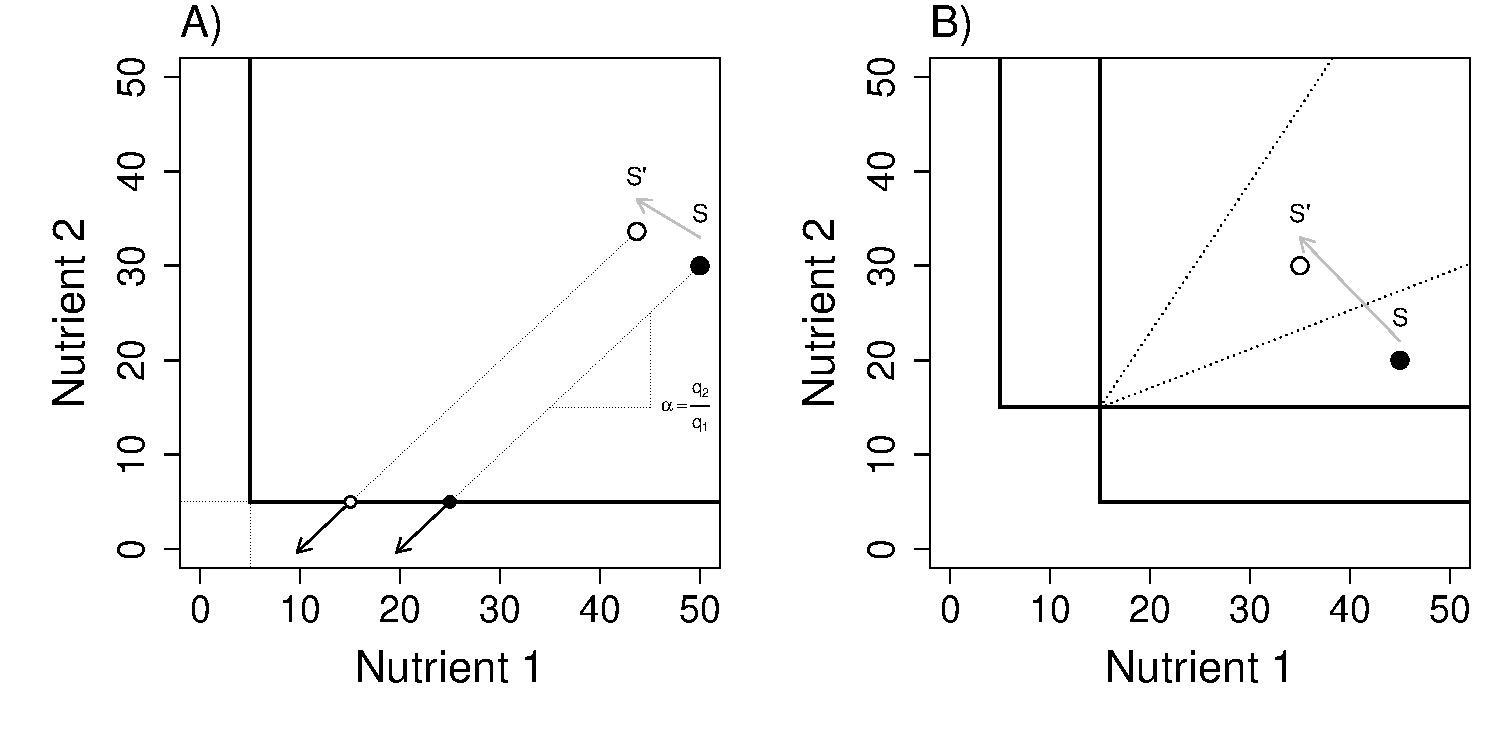
\includegraphics[width=\textwidth]{R-Ratio_theory.pdf}
   \caption{Graphical interpretation of the resource-ratio theory for a single location. The panel A) schematizes the equilibrium state of the system with a single resident primary producer population. Nutrient cycling moves the location of the supply point, from location $S$ to the location $S’$. At equilibrium, the consumption vector is opposed to a net nutrient supply vector. The location of the equilibrium nutrient concentration will only be affected if the slope of the net supply vector is different of the slope of the consumption vector. Panel B) illustrates the conditions for coexistence. A second species could invade the system if its ZNGI is below the equilibrium nutrient concentration in the presence of the resident species. The equilibrium nutrient concentration would thus be found at the crossing of the two ZNGIs. Stable coexistence will occur if the location of the net supply points is found between the projection of the two consumption vectors (dotted lines) and if each species is more limited by the nutrient it requires the most (in other words, if the slope of the consumption vector increases as the ZNGI moves up and left).}
   \label{f:R-Ratio_theory}
\end{figure}
\newpage

\begin{figure}[p]
   \centering
   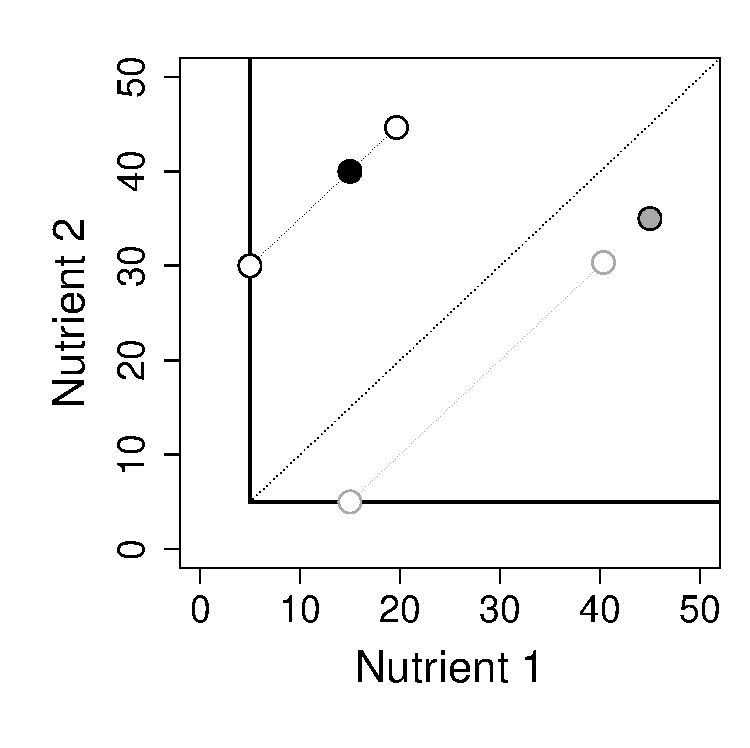
\includegraphics[width=0.45\textwidth]{DetritusDiffusion.pdf}
   \caption{Impacts of detritus diffusion on the equilibrium states of the metaecosystem with a single resident primary producer species. The filled symbols represent the original supply points (inorganic nutrient concentration in absence of consumption) while the open symbols represent the equilibrium quantities when accounting for consumption, recycling and diffusion. The figure shows that the net supply rate of both nutrients increases at the least productive location (in black) while it decreases at the least productive location (in grey). A liner functional response of the form $g_{ij}(N_{j}) = \beta_{ij}N_j$ was used. Parameters are: $e=0.1$, $r= 0.5$, $\phi=0.5$, $q_1 = 0.5$, $N^*_1=5$, $N^*_2=5$, $m =0.1$, $\beta_1 = mq_1/N^*_1$, $\beta_2 = mq_2/N^*_2$, $d_N = 0$, $d_P = 0$ and $d_D = 1$.
}
   \label{f:Detritus}
\end{figure}
\newpage

\begin{figure}[p]
   \centering
   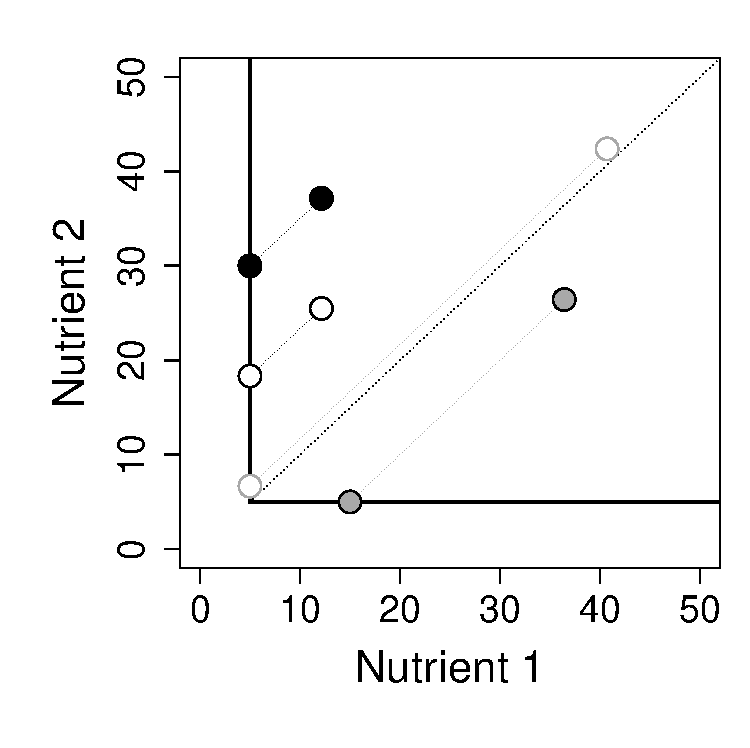
\includegraphics[width=0.45\textwidth]{NutrientDiffusion.pdf}
   \caption{Impacts of inorganic nutrient dispersal on the equilibrium states of the metaecosystem with a single resident primary producer species. Same parameters as the Figure 2, except $r = 0.5$, $d_N = 0.1$, $d_P = 0$ and $d_D = 0$.}
   \label{f:Nutrients}
\end{figure}
\newpage

\begin{figure}[p]
   \centering
   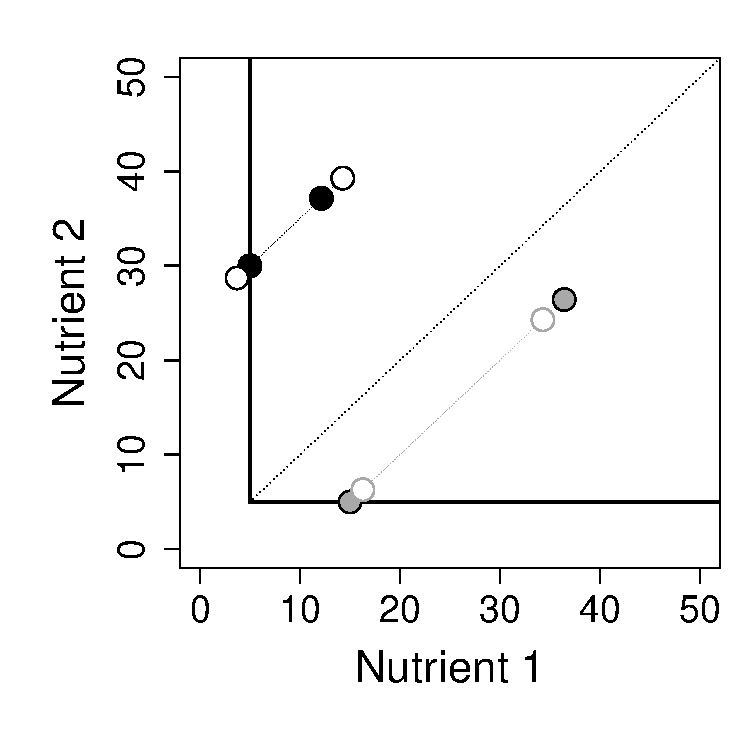
\includegraphics[width=0.45\textwidth]{ProducerDiffusion.pdf}
   \caption{Impacts of primary producer dispersal on the equilibrium states of the metaecosystem with a single resident primary producer species. Same parameters as the Figure 3, except $d_N = 0$, $d_P = 10$ and $d_D = 0$.}
   \label{f:Producers}
\end{figure}
\newpage

\begin{figure}[p]
   \centering
   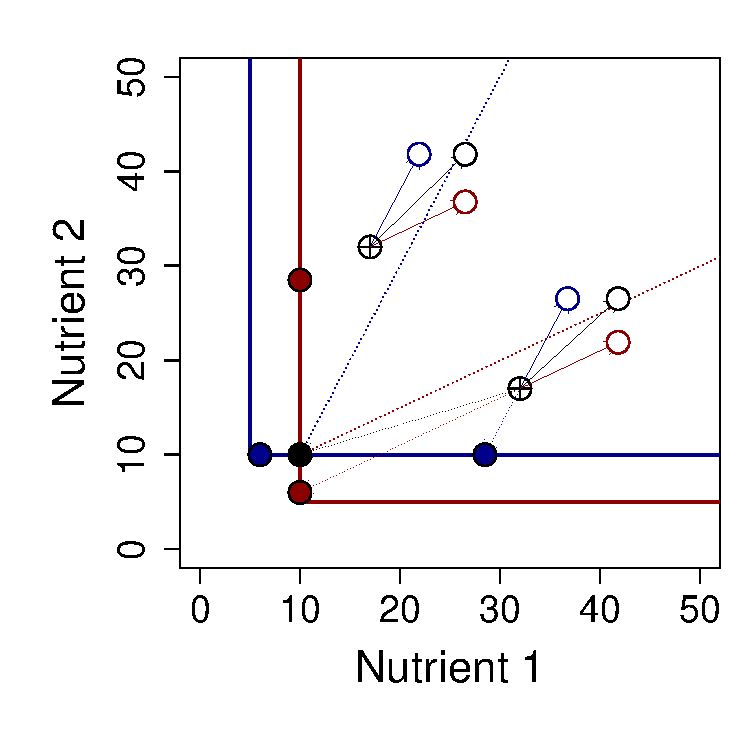
\includegraphics[width=0.45\textwidth]{AlternateStates.pdf}
   \caption{Detritus dispersal could potentially lead to alternate stable states, including locally stable coexistence and locally stable dominance of a single primary producer species. Parameters are: $e=0.1$, $r= 0.1$, $\phi=0.9$, $q_{11} = 1/3$, $N^*_{11}=5$, $N^*_{12}=10$, $m_1 =0.1$, $\beta_{11} = m_1q_{11}/N^*_{11}$, $\beta_{12} = m_1q_{12}/N^*_{12}$,$q_{21} = 2/3$, $N^*_{21}=10$, $N^*_{22}=5$, $m_2 =0.1$,$\beta_{21} = m_2q_{21}/N^*_{21}$, $\beta_{22} = m_2q_{22}/N^*_{22}$, $d_N = 0$, $d_P = 0$ and $d_D = 1$}
   \label{f:ASS}
\end{figure}
\newpage



\end{document}